\documentclass[a4paper,10pt]{article}
\usepackage[left=1in,right=1in,top=1in,bottom=1in]{geometry}
\usepackage[english,russian]{babel}
\usepackage{enumitem}
\usepackage[hidelinks]{hyperref}
\usepackage{titlesec}
\usepackage{multirow}
\usepackage{graphicx}
\usepackage{wrapfig}
\usepackage{tabularx}
\usepackage{float}
\usepackage{longtable}
\usepackage{hyperref}
\hypersetup{colorlinks=true,urlcolor=blue}
\usepackage[rgb]{xcolor}
\usepackage{amsmath,amsfonts,amssymb,amsthm,mathtools} 
\usepackage{icomma} 
\mathtoolsset{showonlyrefs=true}
\usepackage{euscript}
\usepackage{mathrsfs}
\usepackage{setspace}
\usepackage{cmap}          
\usepackage{mathtext}         
\usepackage[T2A]{fontenc}      
\usepackage[utf8]{inputenc}      

\titleformat{\section}{\Large\bfseries}{}{0em}{}[\titlerule]
\pagestyle{empty}

\begin{document}

\begin{center}
    \textbf{\LARGE Даниэль Александрович Сахаров} \\
    \vspace{5pt}
    \href{https://github.com/grgtr}{GitHub} $\vert$
    Долгопрудный, Россия $\vert$ 
    sakharov.da@phystech.edu $\vert$ 
    (915) 229 11 82 $\vert$ 
    tg: @xxxgrgtr
\end{center}

\section*{Образование}
\noindent
\textbf{МФТИ} \hfill 2022 - 2026
Высшая Школа Программная Школа ИВТ Долгопрудный, Россия

\section*{Проекты}
\noindent
\subsection*{1 Учебный проект (\href{https://github.com/hsse-distributed-events-team/devents-second-semester}{DistributedEvents})}
Backend developer, Tech writer,
Reviewer \\  
Сбор требований, участие в составлении ТЗ. \\
Обновление и управление версиями. \\
Создание функционала на python Django. \\
Техническая поддержка, оптимизация. \\
Работа с внешними API (конкретно с yandex contest api oauth). \\
Рефакторинг чужого кода. \\
Тестирование сайтов. \\
Написание документации на Sphinx.

\subsection*{2 Учебный проект (\href{https://github.com/VS-CDR/final-project_hsse}{Сервис такси})}
Backend developer \\
Работа с docker, mongodb, postgres. \\
Проект - система микросервисов на Go. \\
Покрытие наблюдаемостью. \\
Работа с kafka, jaeger. \\
Концепция чистой архитектуру.


\section*{Навыки}
\noindent
\begin{itemize}[noitemsep]
    \item Алгоритмы, теоритические навыки: Базовые структуры данных (и некоторые их реализации на \href{https://github.com/grgtr/MIPT-CPP}{с++}), cортировки, кучи, Sparse Table, ДО, Фенвик, Хеш-таблицы, Деревья поиска, Динамическое программирование, Обходы графов, Кратчайшие пути, Остовы, паросочетания, потоки, Простые строковые алгоритмы (префикс и z функция, бор, Ахо-Корасик), Сложные строковые алгоритмы (суфф массив, дерево, автомат, массив LCP, Теория чисел и FFT, Геометрия (триангуляции, построение выпуклой оболочки 2D и 3D, сумма минковского, диаграмма Вороного, граф Делоне)) \\
    \href{https://gitlab.com/grgtr}{Задачи}, которые проходили ревью в течение курса
    \item C++: ООП, Шаблоны, Наследование, Полиморфизм и виртуальные функции, Исключения, Контейнеры и итераторы, Аллокаторы и управление памятью, Move-семантика и rvalue-ссылки, Умные указатели, Лямбда-функции и элементы функционального программирования, Шаблонное метапрограммирование, SFINAE и концепты
    \item ML: Стандартные задачи машинного обучения: классификация, регрессия и кластеризация. Обучение с учителем и без учителя. Метрики качества и функции потерь. Недообучение и переобучение, кривые обучения. Кросс-валидация и ее виды. Параметры и гипер-параметры алгоритмов.
    SVM и Kernel trick.
    Решающие деревья и ансамбли.
    Бэггинг и бустинг.
    Градиентный бустинг над деревьями.
    Метрики оффлайн качества в задачах обучения с учителем.
    SGD и его модификации для нейронных сетей.
    Нейронные сети. Принцип работы и матричная запись. 
    И ещё пару тем.
    \item GO: Архитектура систем, Документация и тестирование, Наблюдаемость, Нереляционные БД, MongoDB, Реляционные БД, PostgresSQL, Асинхронное взаимодействие, Kafka/Rabbit/NATS, Docker
    \item Python: NumPy, Pandas, scikit-learn, TensorFlow
    \item Администрирование Линукс, git (23/23 git exercises), html, css, javascript, React
    \item Мат. навыки: отлично знаю программу по мат.анализу(сдавал комиссию), линейную алгебру знаю хорошо(но многих доказательств уже не смогу вывести), особое внимение уделил курсам Теории вероятности и Дифф. уравнениям
\end{itemize}

\section*{Дополнительная информация}
\noindent
\textbf{Достижения:} \\ призёр многих олимпиад по математике, физике, могу выделить физтех физику и математику 2021 и 2022 года, участвую время от времени в очных хакатонах по робототехнике, криптографии


\begin{center}
  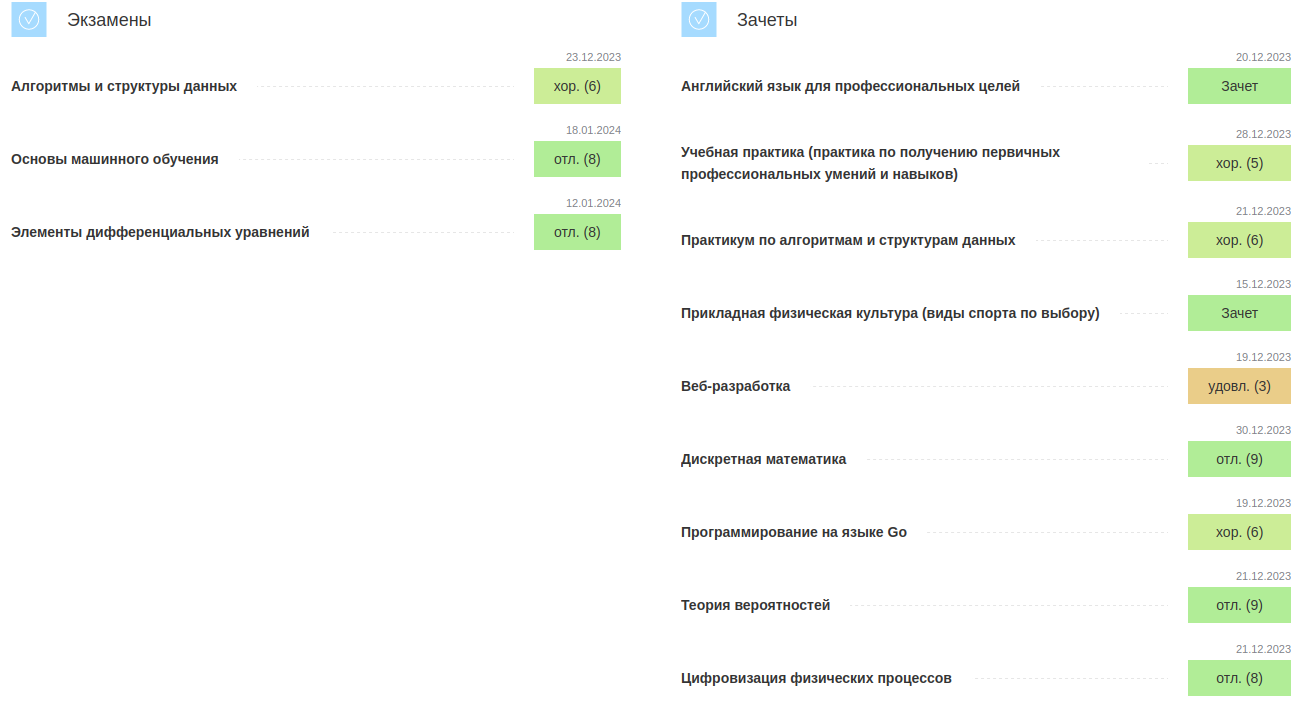
\includegraphics[scale = 0.5]{pic1.png}
\end{center}

\end{document}
